\chapter{\ifproject%
\ifenglish Experimentation and Results\else การทดลองและผลลัพธ์\fi
\else%
\ifenglish System Evaluation\else การประเมินระบบ\fi
\fi}
\hspace{10mm} จากการทดลองนำกล้อง ESP32-CAM with OV2640 ไปติดตั้งบริเวณชั้น 2 ของสำนักหอสมุดมหาวิทยาลัยเชียงใหม่จำนวน 3 โซน เพื่อตรวจสอบจำนวนคนที่มีอยู่โดยใช้ AWS Rekcognition ผลเป็นดังนี้

\section{การทดลองโซนที่ 1}
\begin{figure}[ht]
    \centering
    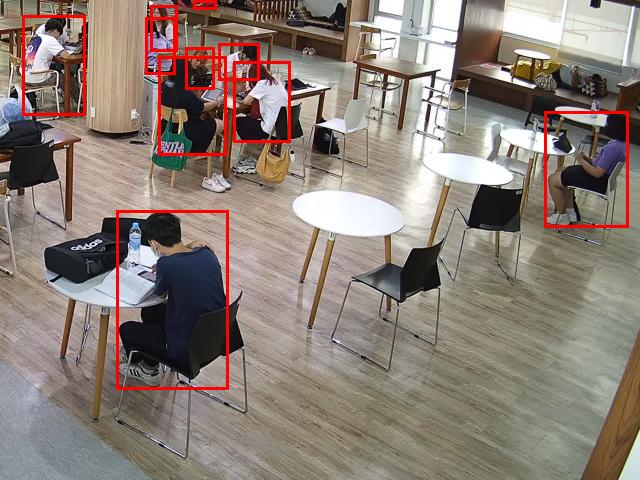
\includegraphics[scale=0.5]{images/modified_Picture (100).jpg}
    \caption[output1]{ตัวอย่าง output ที่ได้จากการติดตั้งกล้องโซนที่ 1}
    \label{fig:output1}
\end{figure}
\begin{figure}[ht]
    \centering
    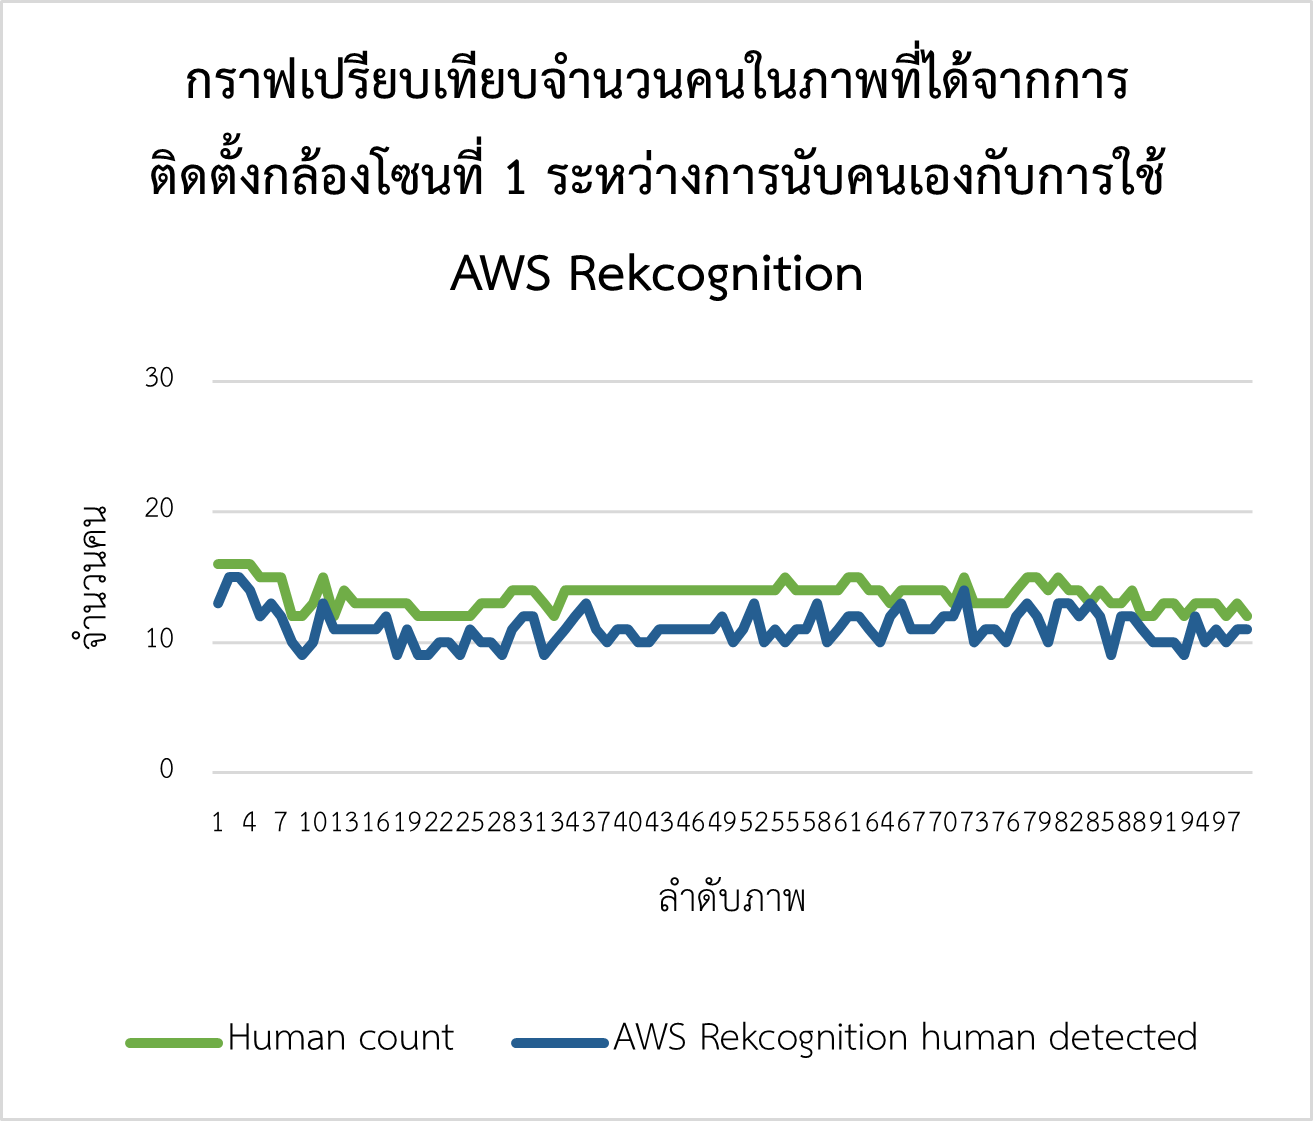
\includegraphics[scale=1]{images/graph1_zone1.png}
    \caption[graph1-1]{กราฟเปรียบเทียบจำนวนคนในภาพที่ได้จากการติดตั้งกล้องโซนที่ 1 ระหว่างการนับคนเองกับการใช้ AWS Rekcognition}
    \label{fig:graph1-1}
\end{figure}
\begin{figure}[ht]
    \centering
    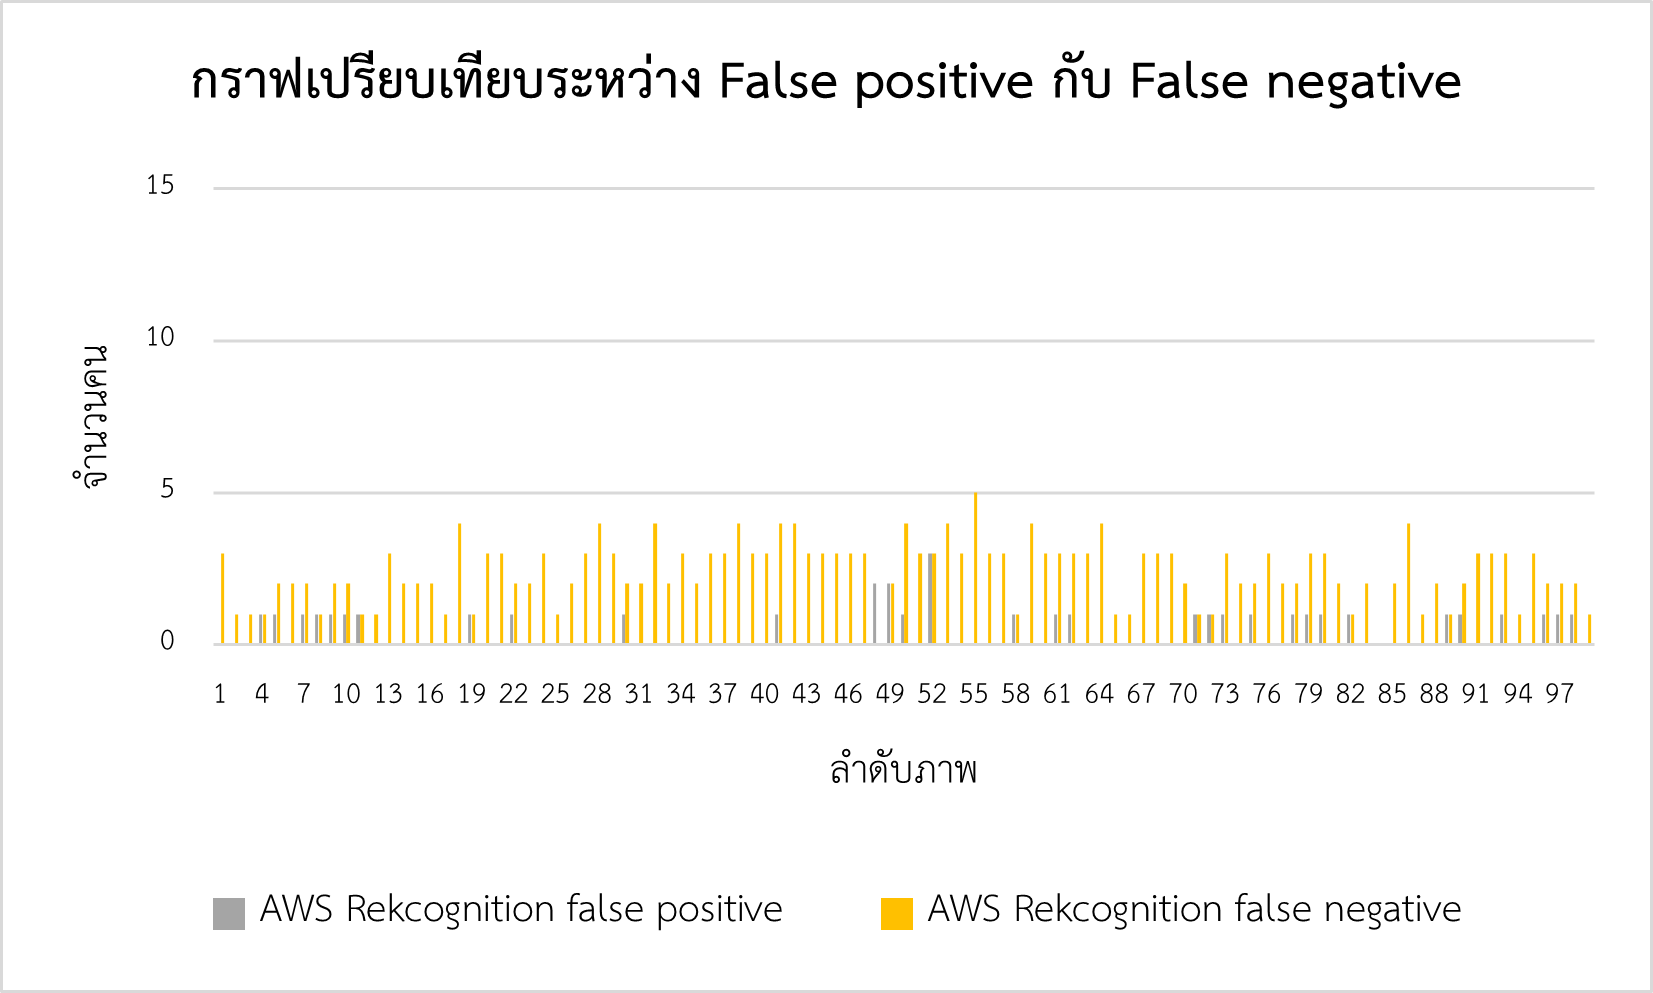
\includegraphics[scale=1]{images/graph2_zone1-2.png}
    \caption[graph2-1]{กราฟเปรียบเทียบระหว่าง False positive กับ False negative}
    \label{fig:graph2-1}
\end{figure}
จากภาพทั้งหมด 99 ภาพ พบว่า Accuracy คือ 0.82 มี False positive และ False negative ปานกลาง

\section{การทดลองโซนที่ 2}
\begin{figure}[ht]
    \centering
    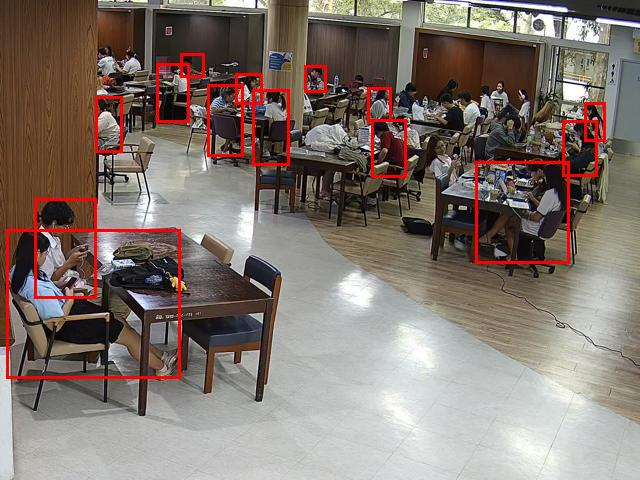
\includegraphics[scale=0.5]{images/modified_Picture (102).jpg}
    \caption[output2]{ตัวอย่าง output ที่ได้จากการติดตั้งกล้องโซนที่ 2}
    \label{fig:output2}
\end{figure}
\begin{figure}[ht]
    \centering
    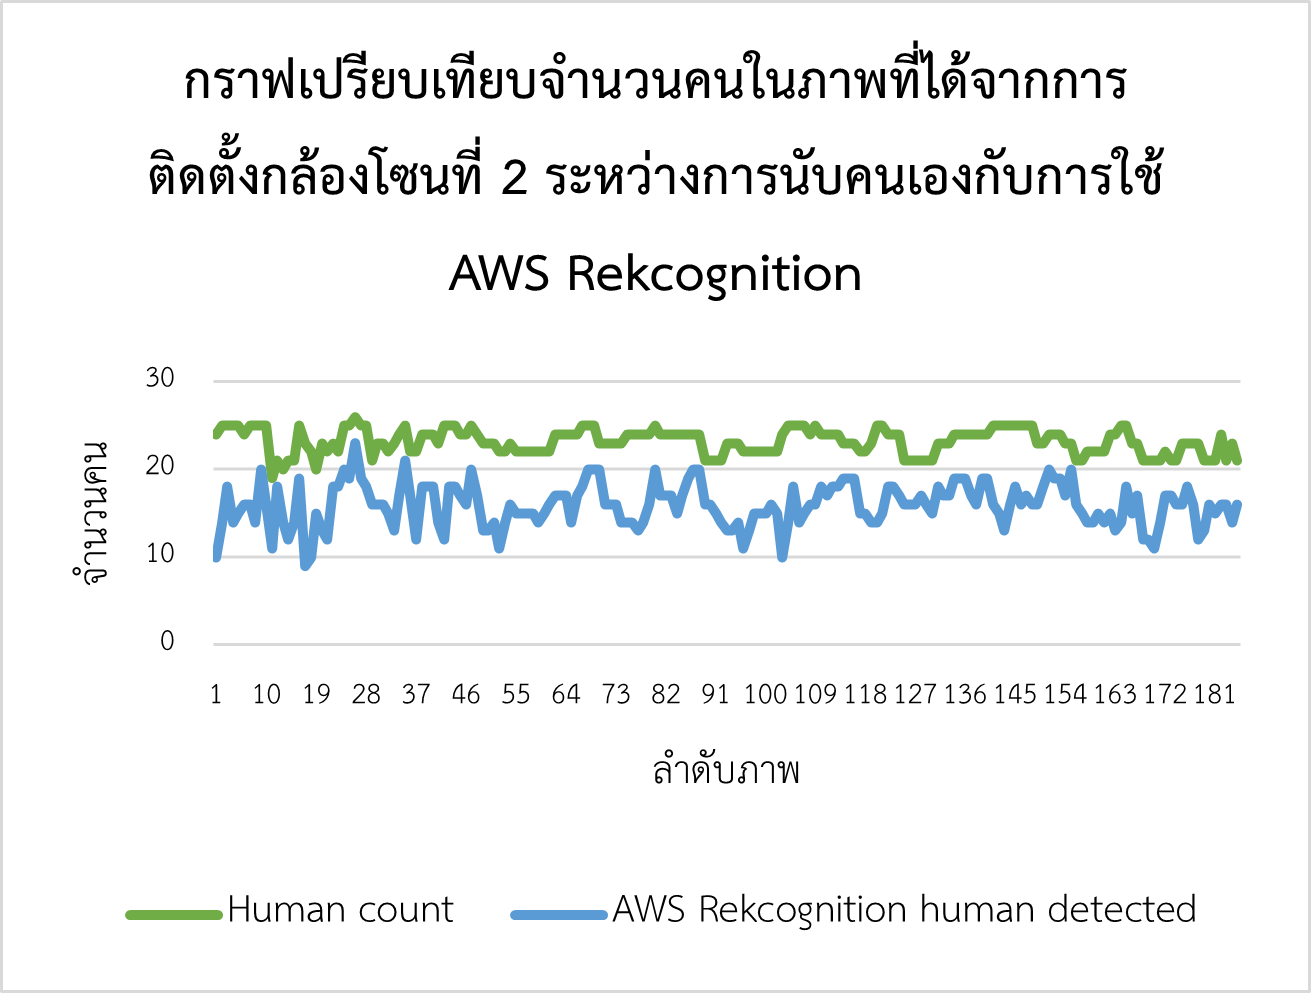
\includegraphics[scale=1]{images/graph1_zone2.png}
    \caption[graph1-2]{กราฟเปรียบเทียบจำนวนคนในภาพที่ได้จากการติดตั้งกล้องโซนที่ 2 ระหว่างการนับคนเองกับการใช้ AWS Rekcognition}
    \label{fig:graph1-2}
\end{figure}
\begin{figure}[ht]
    \centering
    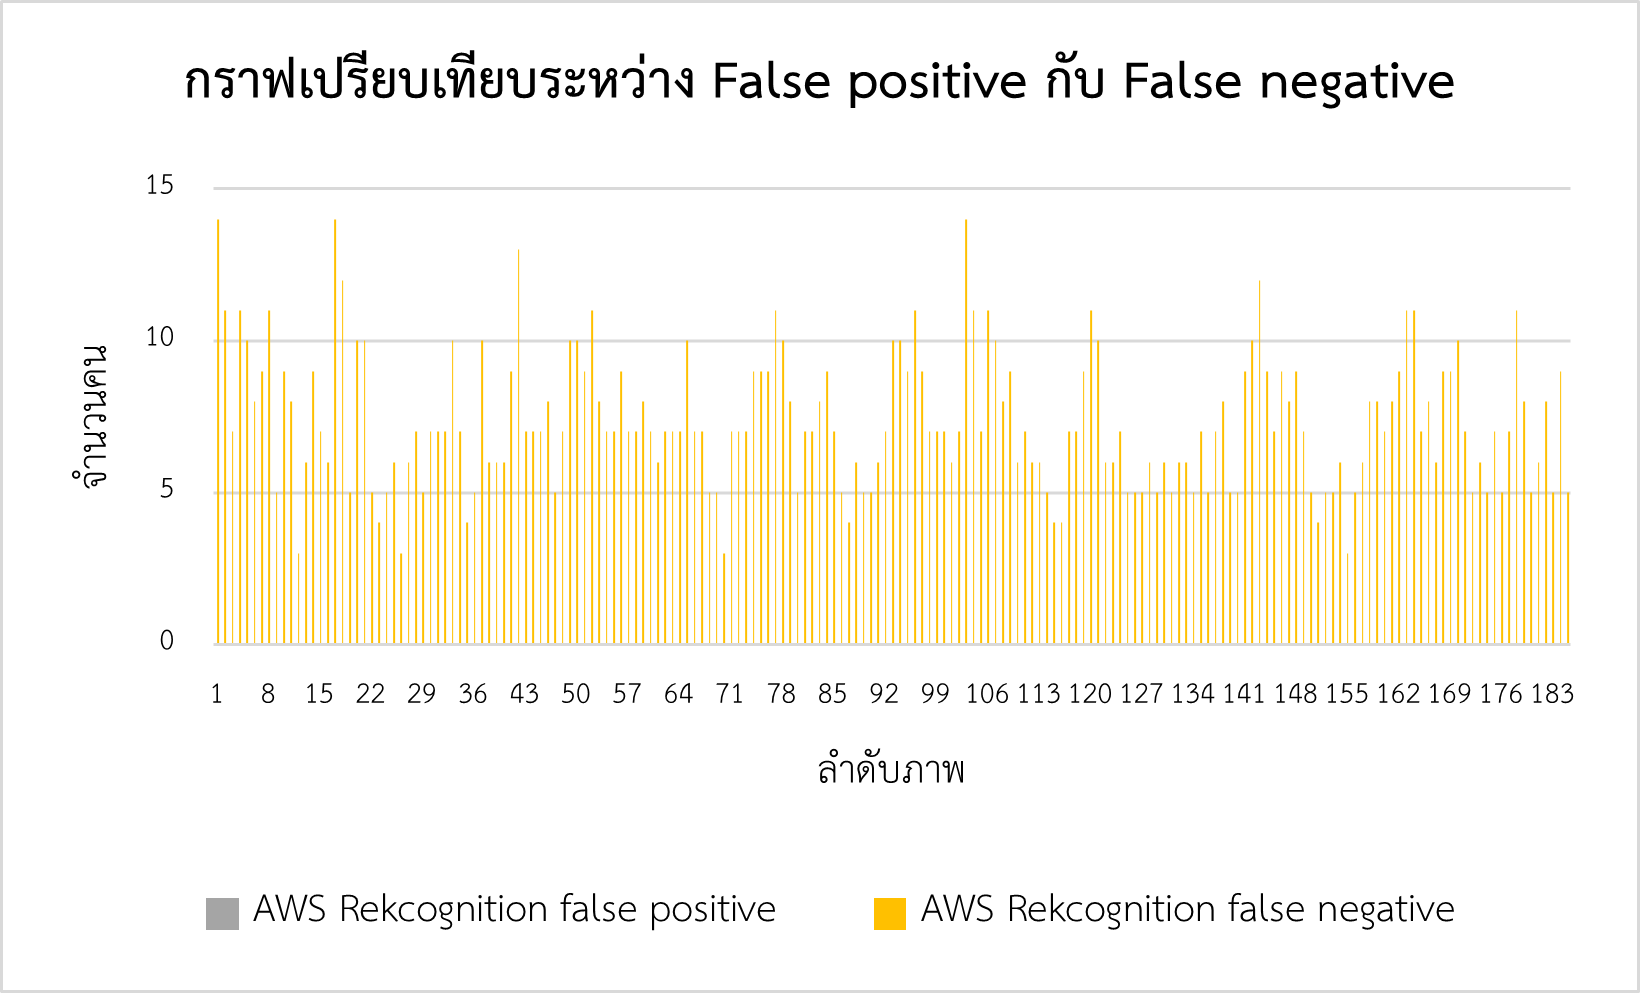
\includegraphics[scale=1]{images/graph2_zone2.png}
    \caption[graph2-2]{กราฟเปรียบเทียบระหว่าง False positive กับ False negative}
    \label{fig:graph2-2}
\end{figure}
จากภาพทั้งหมด 185 ภาพ พบว่า Accuracy คือ 0.69 ไม่มี False positive ส่วน False negative สูง

\section{การทดลองโซนที่ 3}
\begin{figure}[ht]
    \centering
    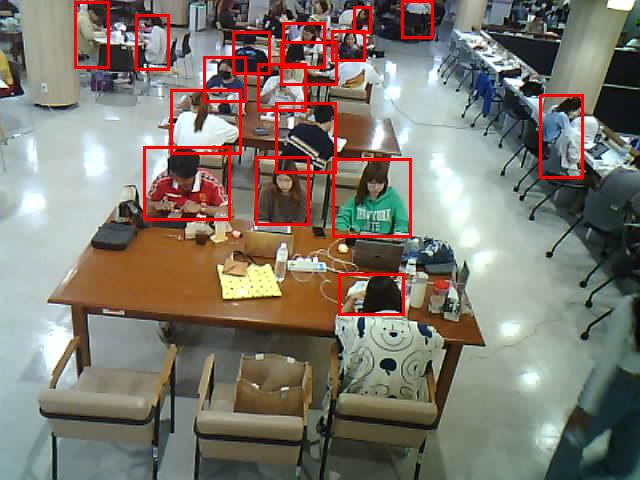
\includegraphics[scale=0.5]{images/modified_ESP32-CAM(26).jpg}
    \caption[output3]{ตัวอย่าง output ที่ได้จากการติดตั้งกล้องโซนที่ 3}
    \label{fig:output3}
\end{figure}
\begin{figure}[ht]
    \centering
    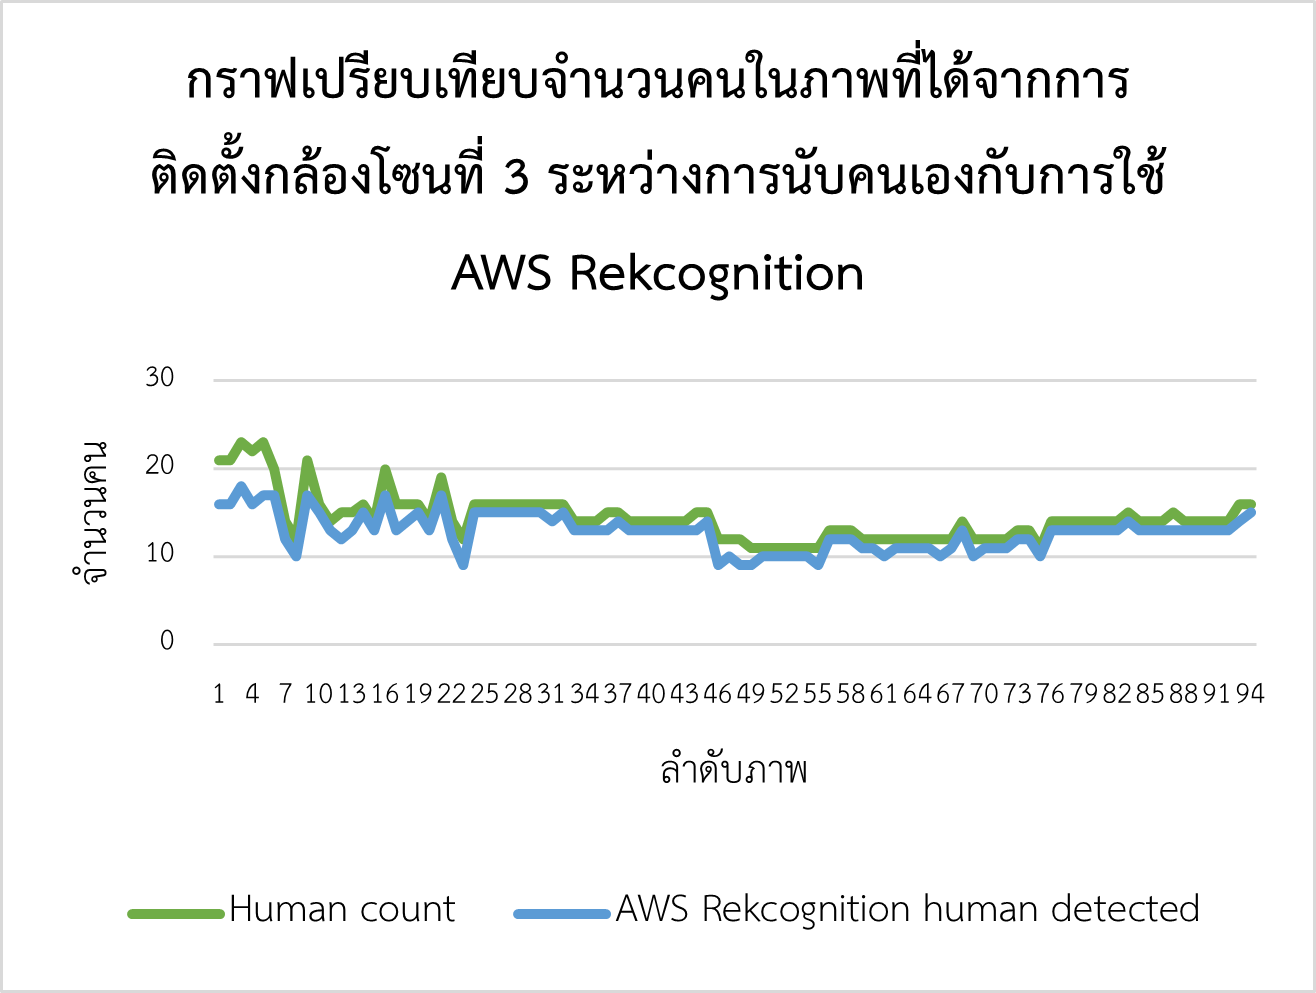
\includegraphics[scale=1]{images/graph1_zone3.png}
    \caption[graph1-3]{กราฟเปรียบเทียบจำนวนคนในภาพที่ได้จากการติดตั้งกล้องโซนที่ 3 ระหว่างการนับคนเองกับการใช้ AWS Rekcognition}
    \label{fig:graph1-3}
\end{figure}
\begin{figure}[ht]
    \centering
    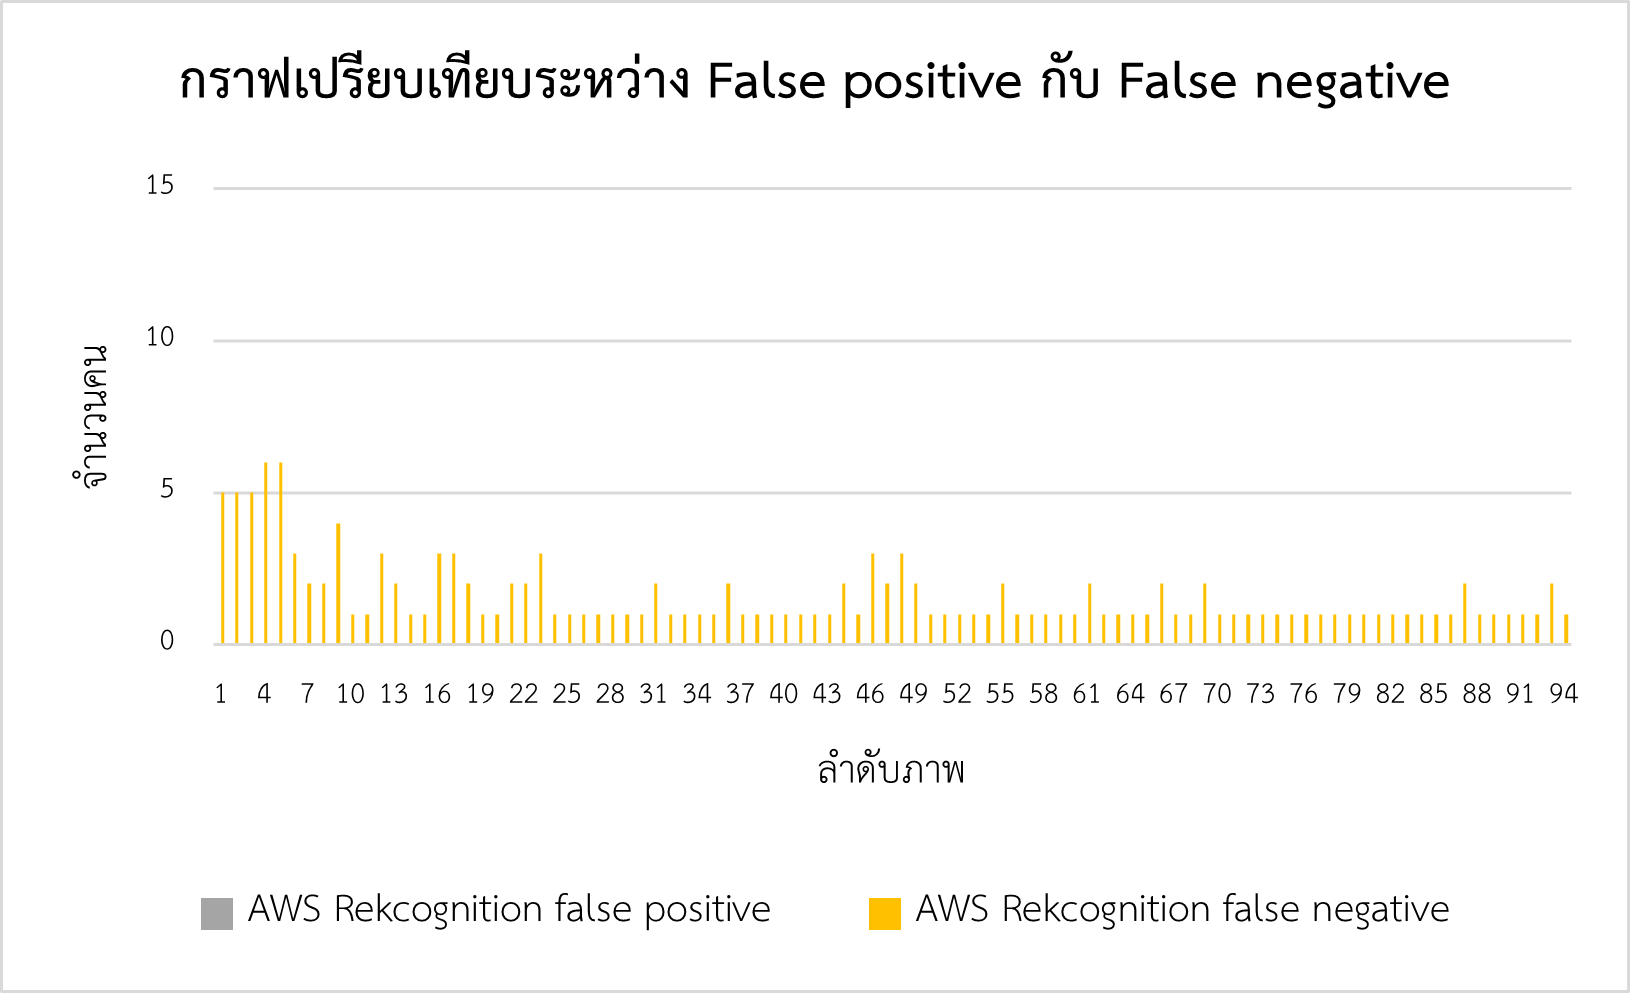
\includegraphics[scale=1]{images/graph2_zone3-2.png}
    \caption[graph2-3]{กราฟเปรียบเทียบระหว่าง False positive กับ False negative}
    \label{fig:graph2-3}
\end{figure}
จากภาพทั้งหมด 94 ภาพ พบว่า Accuracy คือ 0.89 ไม่มี False positive ส่วน False negative ต่ำ

\section{ตารางเปรียบเทียบผลที่ได้จากทั้ง 3 โซน}
\begin{figure}[ht]
    \centering
    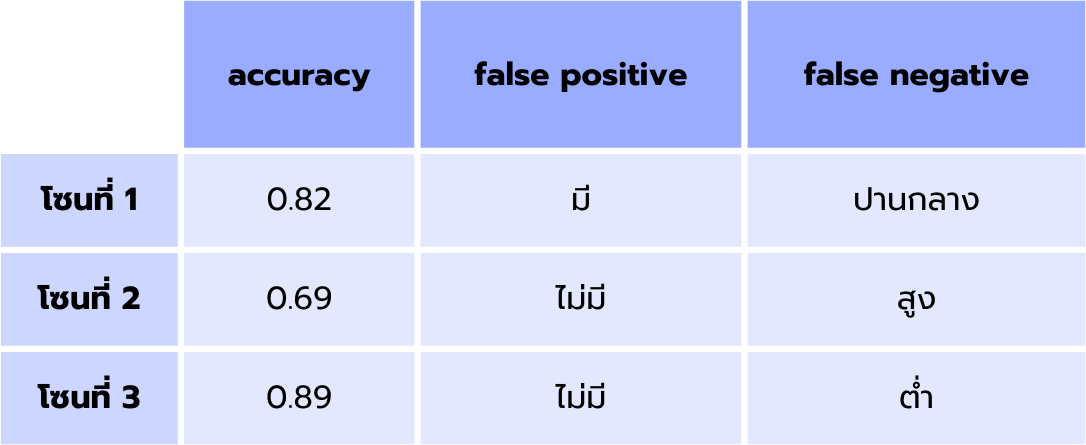
\includegraphics[scale=0.5]{images/comparison.png}
    \caption[comparison]{ตารางเปรียบเทียบผลที่ได้จากทั้ง 3 โซน}
    \label{fig:comparison}
\end{figure}
AWS Rekcognition สามารถทํางานได้มีประสิทธิภาพมากยิ่งขึ้นหากได้ภาพจากกล้องที่มีตําแหน่งเหมาะสม เห็นคนชัด ไม่มีจุดที่สังเกตได้ยาก หรือมุมกล้องที่ไกลเกินไปที่จะ
ทําให้ความมั่นใจในการตรวจจับคนลดลง โดยมีแนวทางการติดตั้งกล้อง 1 ตัวต่อ 2-3 โต๊ะ
โดยที่จะต้องเห็นคนนั่งห่างกันในมุมสูง

\section{ผลการประเมินความพึงพอใจ}
แบบประเมินความพึงพอใจจะประเมินอยู่ทั้งหมด 3 ด้าน คือ ด้านความง่ายต่อการใช้งาน (Usability), ด้านประสิทธิภาพ (Perfomance) และด้านตรงตามความต้องการ (Function Requirement) โดยแบ่งกลุ่มผู้ประเมินเป็น 2 กลุ่ม คือ จากนักศึกษาจำนวน 15 คนและทางสำนักหอสมุด 2 คน 
และระดับการวัดผลคือ 5 หมายถึง ดีมาก, 4 หมายถึง ดี, 3 หมายถึง ปานกลาง, 2 หมายถึง น้อย และ 1 หมายถึง น้อยที่สุด
\subsection{ผลการประเมินความพึงพอใจจากนักศึกษา}
\begin{figure}[ht]
    \centering
    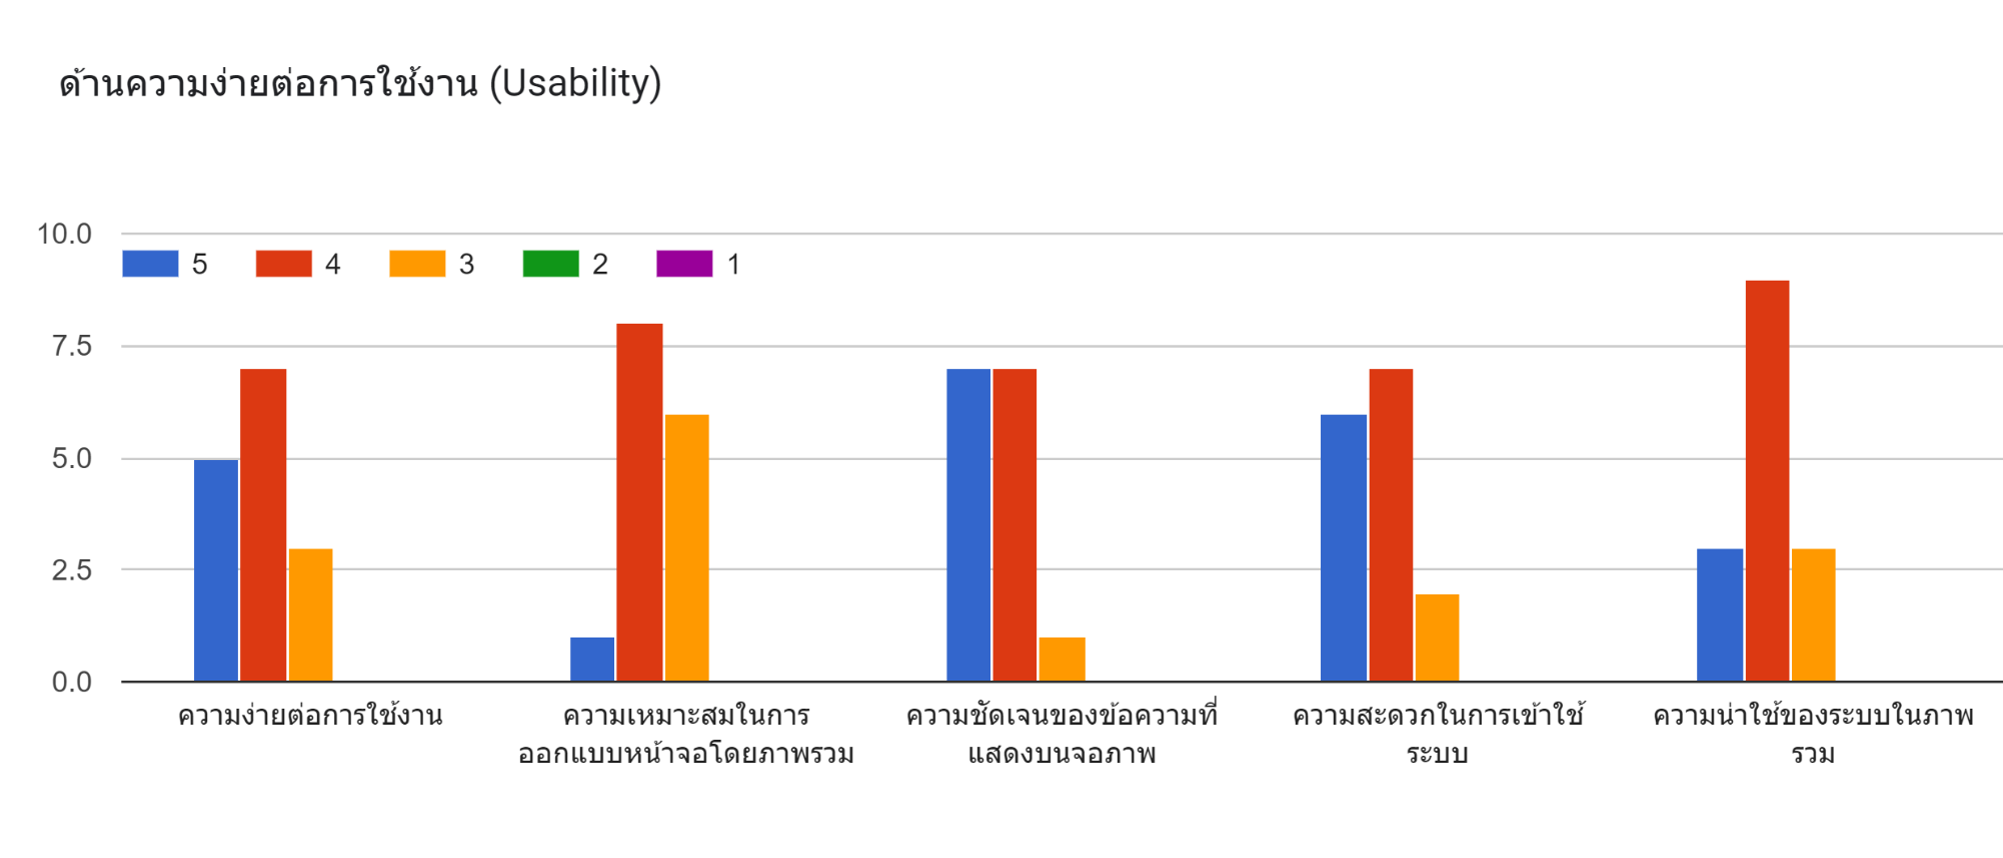
\includegraphics[scale=0.6]{images/student-u.png}
    \caption[st-u]{ผลการประเมินความพึงพอใจของนักศึกษาด้านความง่ายต่อการใช้งาน (Usability)}
    \label{fig:st-u}
\end{figure}
\begin{figure}[ht]
    \centering
    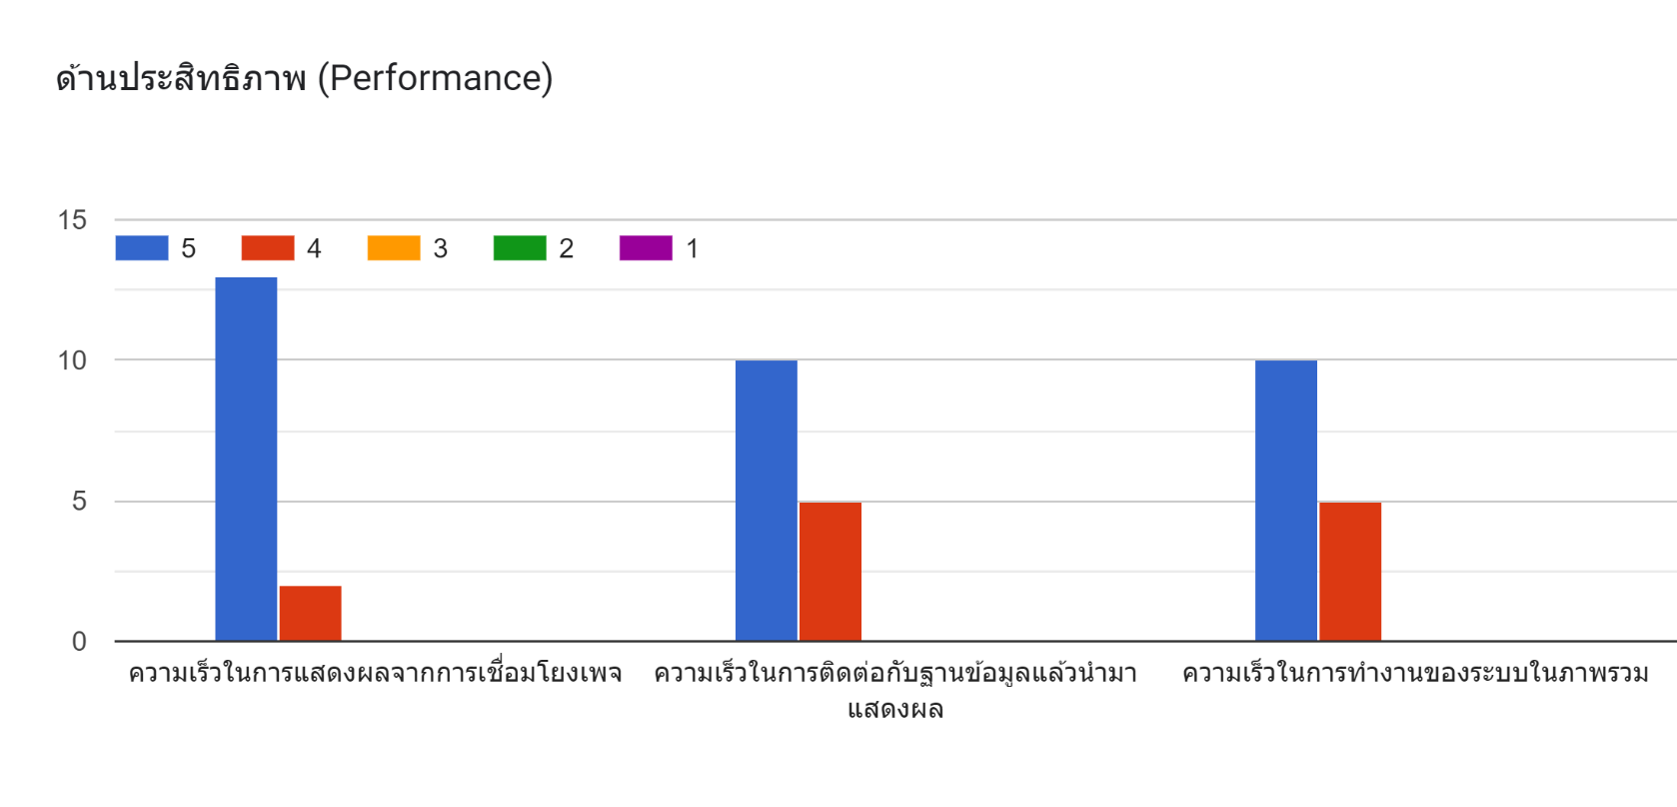
\includegraphics[scale=0.6]{images/student-p.png}
    \caption[st-p]{ผลการประเมินความพึงพอใจของนักศึกษาด้านประสิทธิภาพ (Perfomance)}
    \label{fig:st-p}
\end{figure}
\begin{figure}[ht]
    \centering
    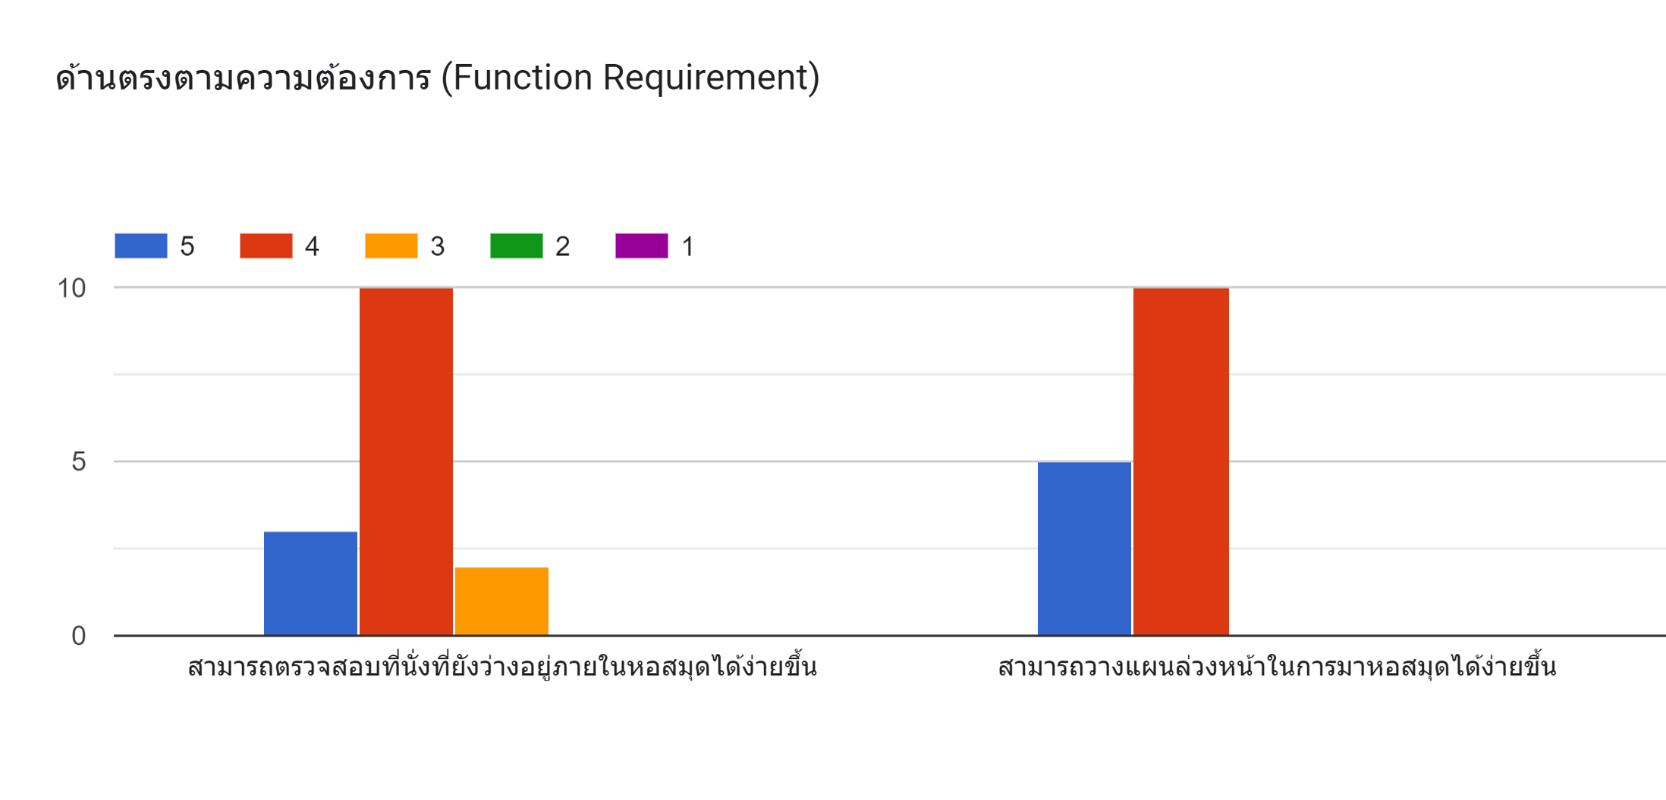
\includegraphics[scale=0.6]{images/student-f.png}
    \caption[st-f]{ผลการประเมินความพึงพอใจของนักศึกษาด้านตรงตามความต้องการ (Function Requirement)}
    \label{fig:st-f}
\end{figure}

\subsection{ผลการประเมินความพึงพอใจจากทางสำนักหอสมุด}
\begin{figure}[ht]
    \centering
    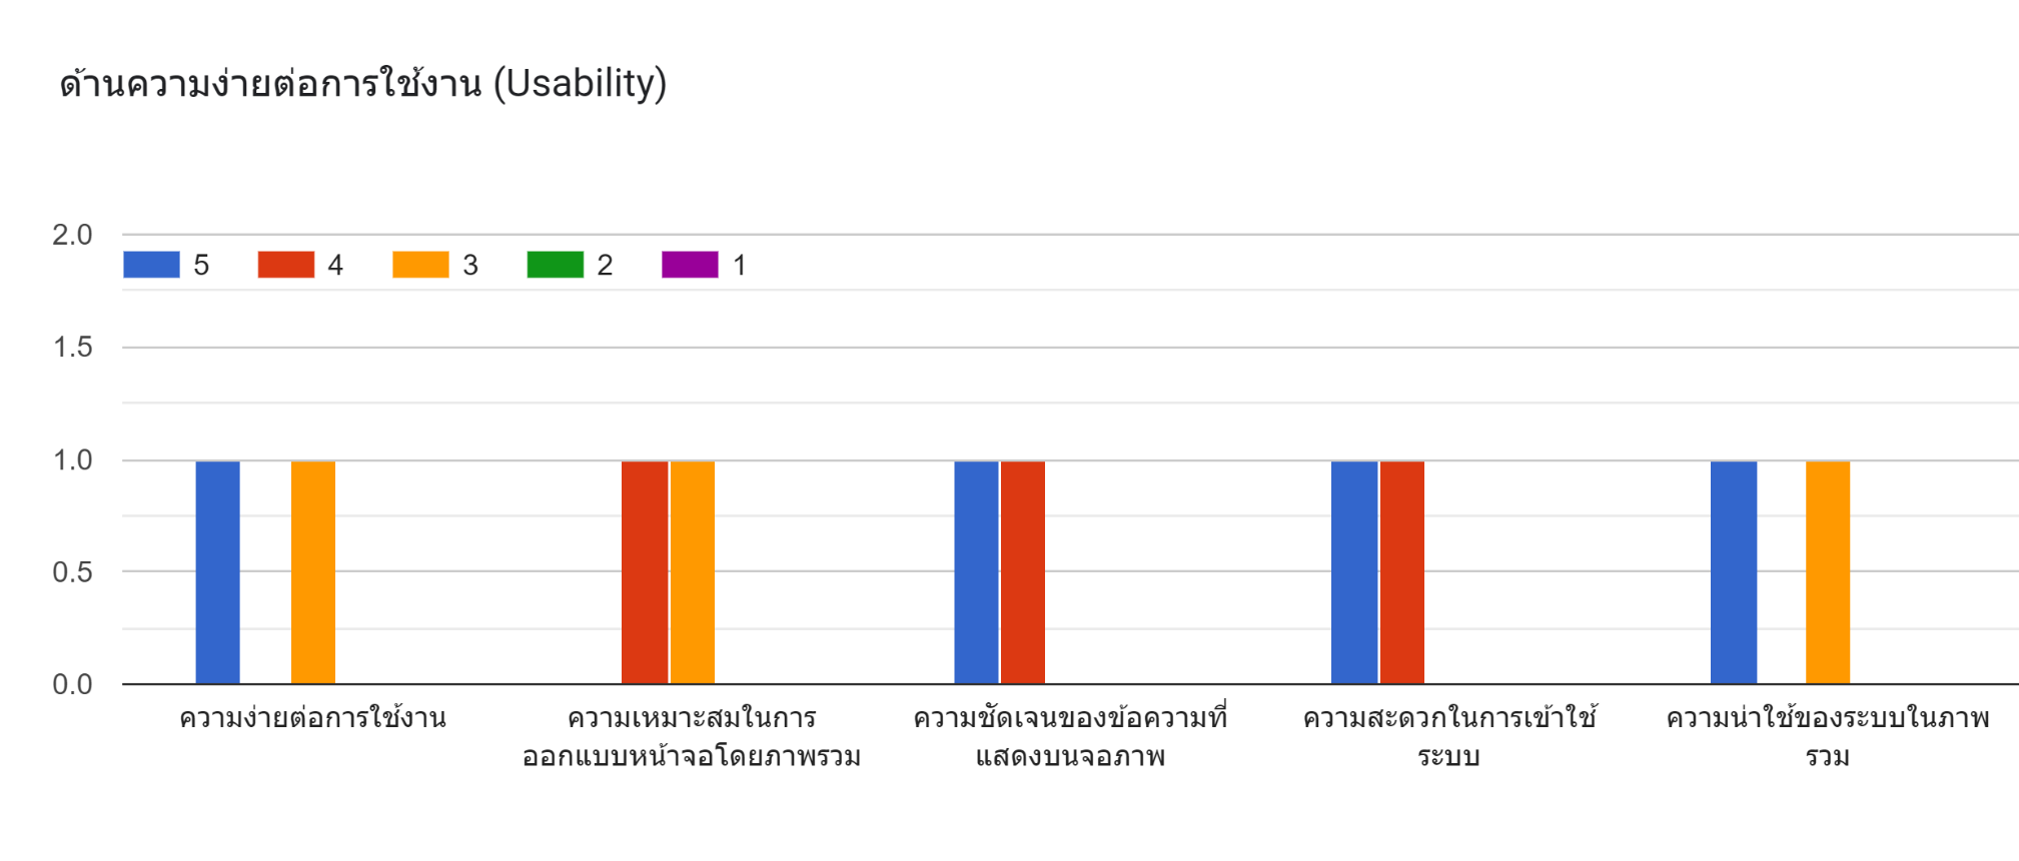
\includegraphics[scale=0.6]{images/cmul-u.png}
    \caption[cmul-u]{ผลการประเมินความพึงพอใจของทางสำนักหอสมุดด้านความง่ายต่อการใช้งาน (Usability)}
    \label{fig:cmul-u}
\end{figure}
\begin{figure}[ht]
    \centering
    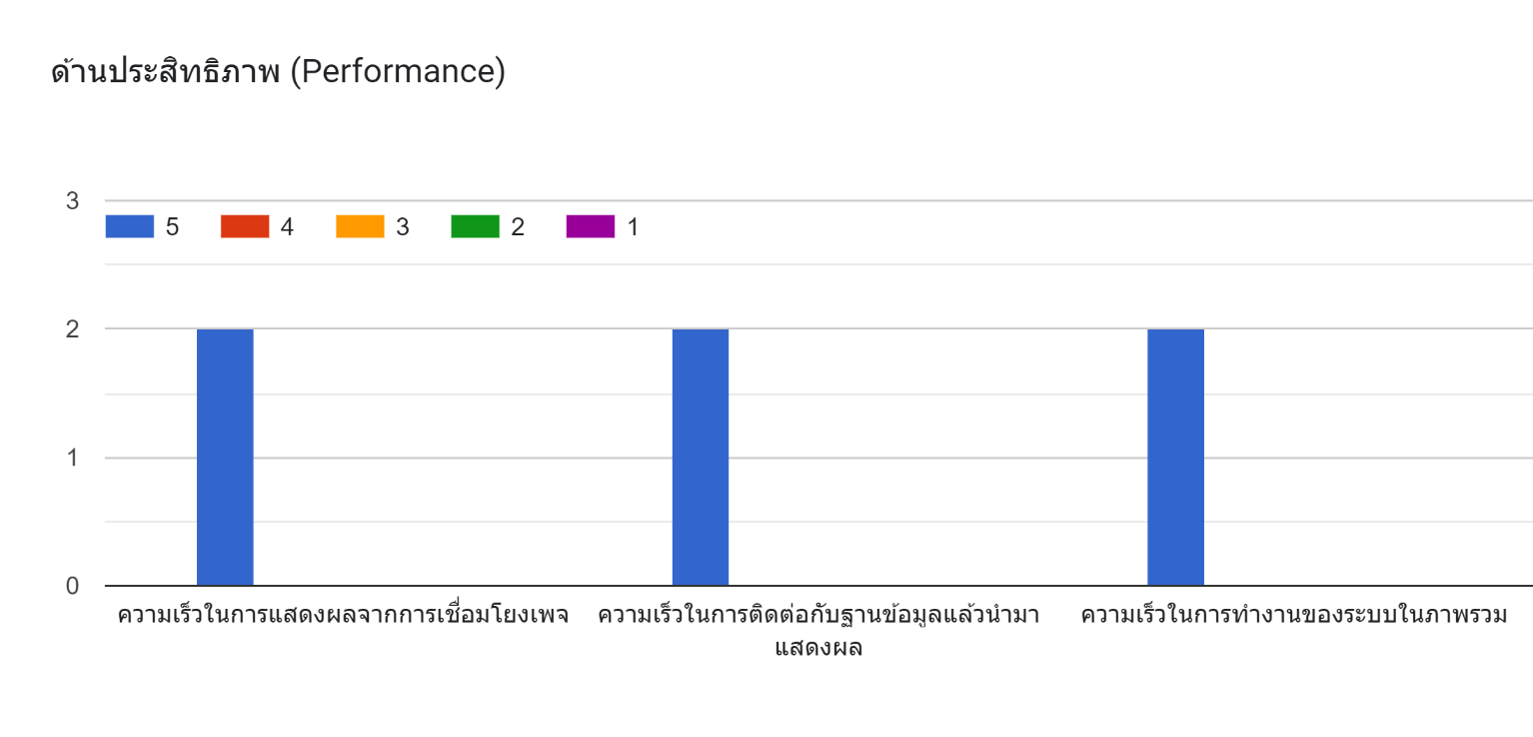
\includegraphics[scale=0.6]{images/cmul-p.png}
    \caption[cmul-p]{ผลการประเมินความพึงพอใจของทางสำนักหอสมุดด้านประสิทธิภาพ (Perfomance)}
    \label{fig:cmul-p}
\end{figure}
\begin{figure}[ht]
    \centering
    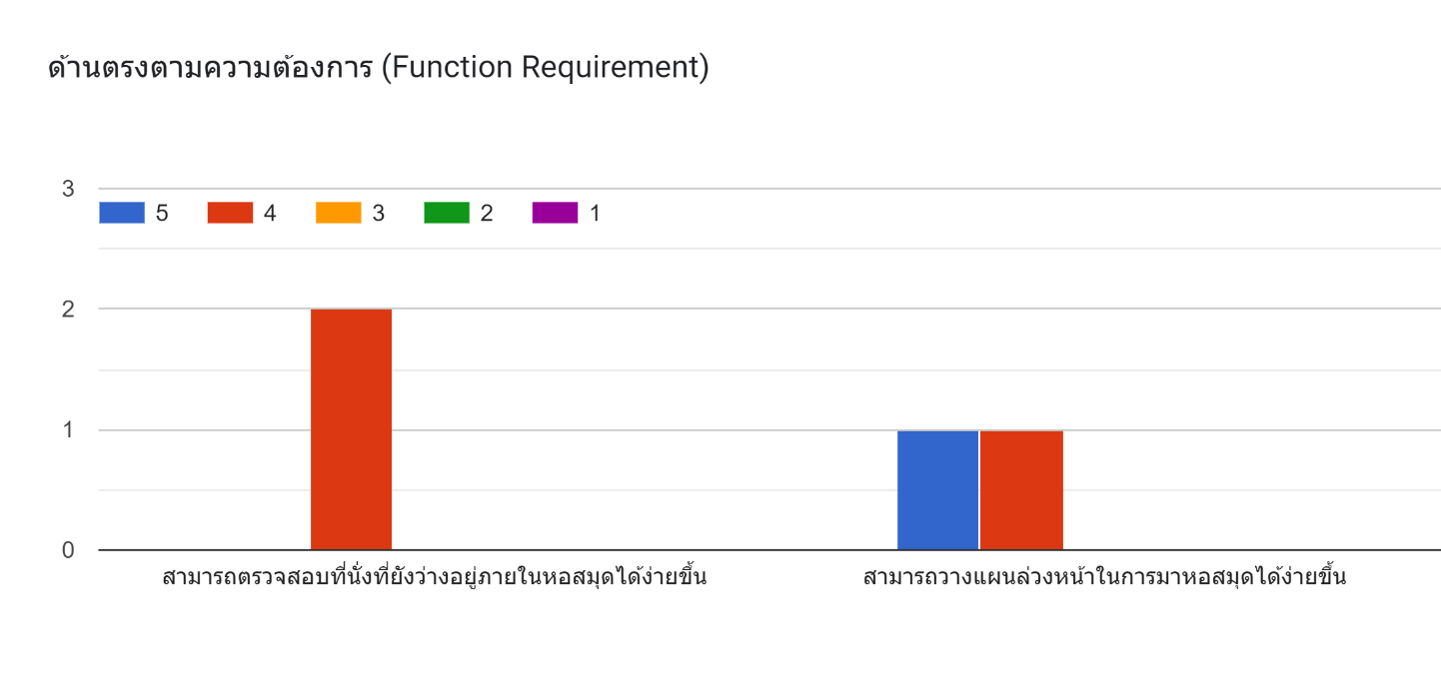
\includegraphics[scale=0.6]{images/cmul-f.png}
    \caption[cmul-f]{ผลการประเมินความพึงพอใจของทางสำนักหอสมุดด้านตรงตามความต้องการ (Function Requirement)}
    \label{fig:cmul-f}
\end{figure}

\subsection{ผลการประเมินความพึงพอใจเฉลี่ยโดยรวม}
\begin{figure}[ht]
    \centering
    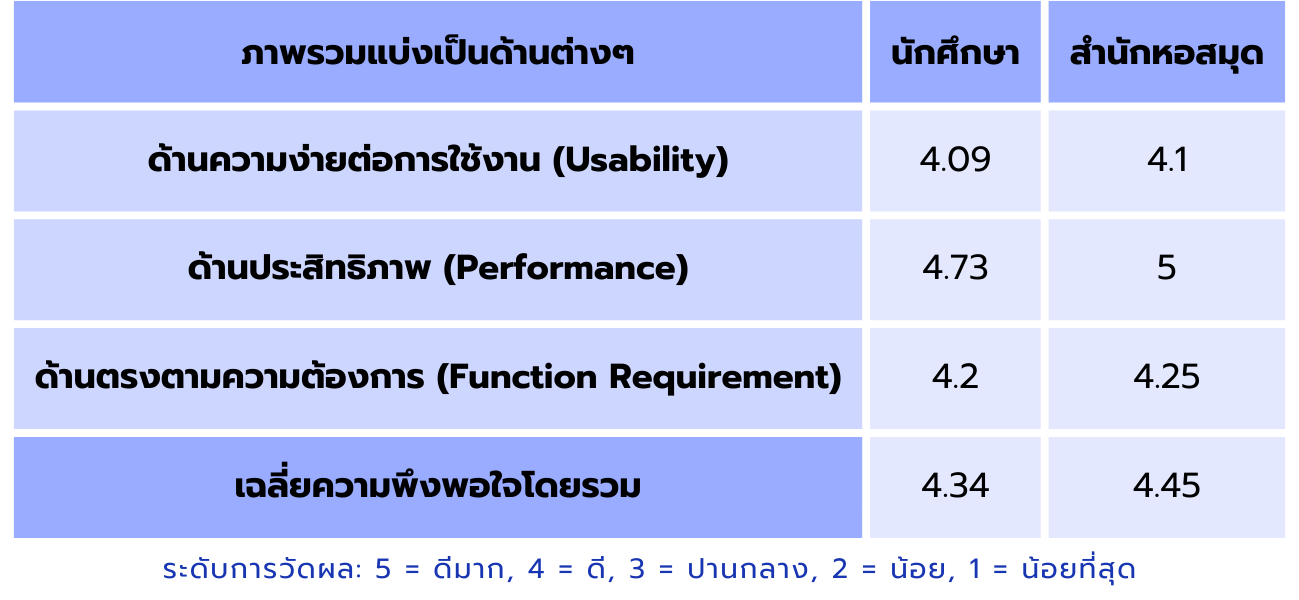
\includegraphics[scale=0.4]{images/satisfaction.png}
    \caption[satisfaction]{ผลการประเมินความพึงพอใจ}
    \label{fig:satisfaction}
\end{figure}
จากนักศึกษาจำนวน 15 คนและทางสำนักหอสมุด 2 คน ได้รับผลประเมินความพึงพอใจโดยรวมเฉลี่ยถือว่าอยู่ในระดับที่ดี
% เนื่องจากมีการนำความรู้เรื่อง Computer Vision มาใช้เกี่ยวกับการทำ Object detection จึงได้มีการศึกษา model และ library
% ของ OpenCV ที่มีให้ทดลองใช้งาน เพื่อเพิ่มความเข้าใจและเลือกใช้ได้อย่างเหมาะสม โดยนำภาพบางส่วนจากการถ่ายรูปสถานที่จริงด้วยกล้องโทรศัพท์มือถือคือบริเวณชั้น 2
% ของสำนักหอสมุดมหาวิทยาลัยเชียงใหม่มาทำการทดสอบจึงมีการทดลองทั้งหมด 3 ครั้ง
% \begin{figure}[ht]
%     \centering
%     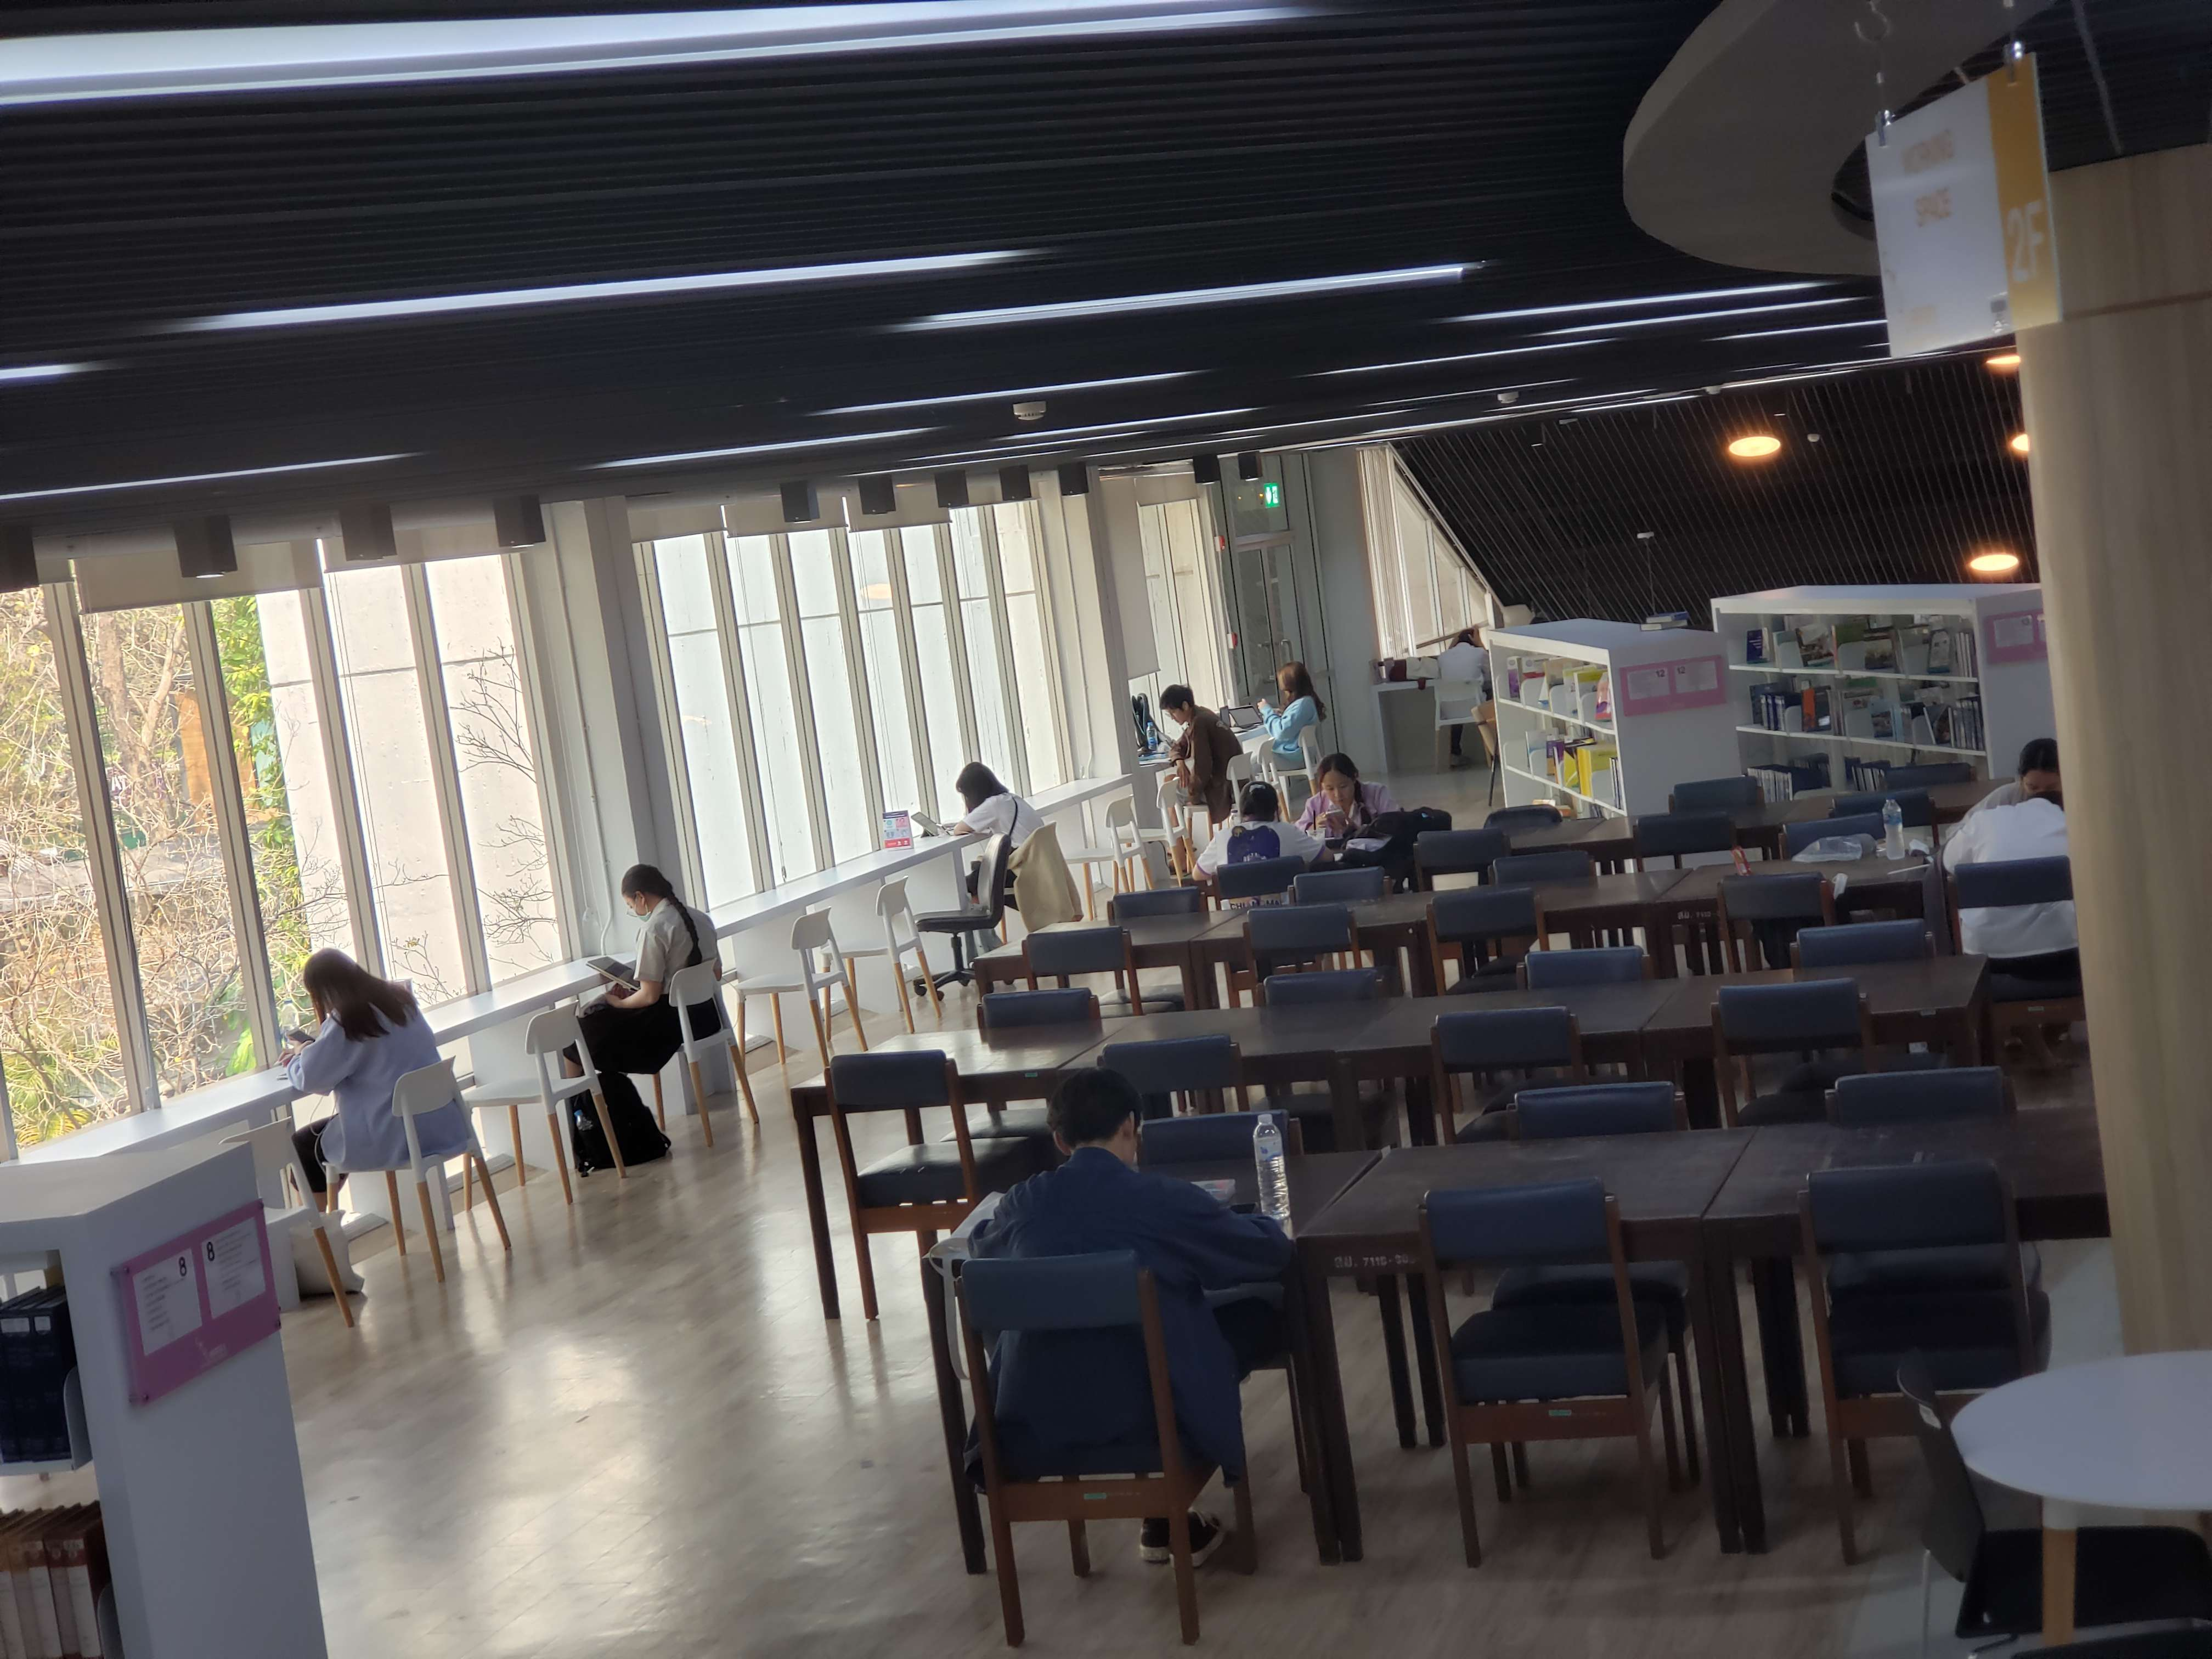
\includegraphics[scale=0.07]{images/cam2-2.jpg}
%     \caption[camera]{ภาพจากกล้องโทรศัพท์มือถือ}
%     \label{fig:camera}
% \end{figure}
% \newpage
% \section{การทดลองครั้งที่ 1 โดยใช้ OpenCV with HOG descriptor}
% \hspace{10mm}HOG (Histograms of Oriented Gradients) descriptor เป็น library ที่ทาง OpenCV มีให้ใช้
% ซึ่งใช้ร่วมกับ SVM Classifier ที่ได้รับการ train มาแล้วจาก cv2.HOGDescriptor\textunderscore getDefaultPeopleDetector()
% ในการจำแนกว่าเป็นคนหรือไม่ใช่คน\cite{OpenHOG}

% \begin{figure}[ht]
%     \centering
%     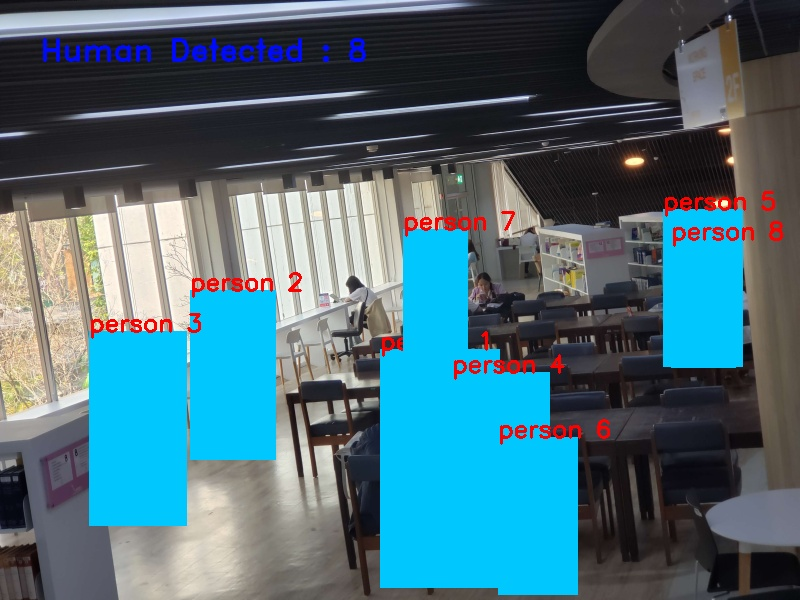
\includegraphics[scale=0.35]{images/hog_output.jpg}
%     \caption[output 1]{output ของการทดลองครั้งที่ 1}
%     \label{fig:output1}
%     \end{figure}

% \hspace{10mm} ผลลัพธ์ที่ได้คือสามารถตรวจจับคนในภาพได้จำนวน 8 คน ซึ่งได้จำนวนมากกว่าความเป็นจริง และตรวจจับได้ในส่วนที่ไม่ใช่คนอีกด้วย
% \newpage
% \section{การทดลองครั้งที่ 2 โดยใช้ OpenCV with Detect common object library}
% \hspace{10mm}Detect common object library เป็น library ที่ทาง OpenCV มีให้ใช้ ซึ่งสามารถตรวจจับวัตถุพื้นฐานได้จาก model YOLOv3 แต่ในการทดลองนี้จะเลือกให้ตรวจจับเฉพาะคนเท่านั้น\cite{OpenYOLO}
% \begin{figure}[ht]
%     \centering
%     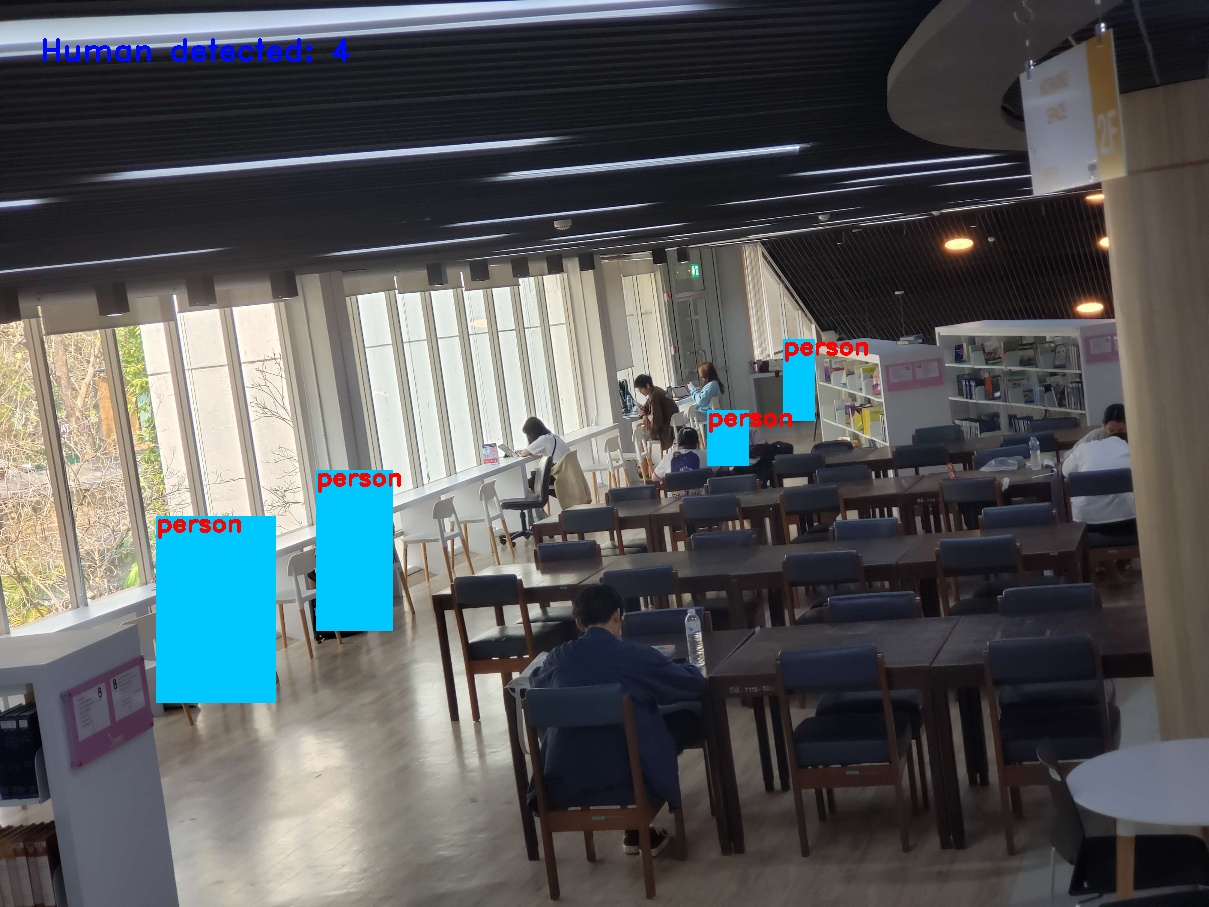
\includegraphics[scale=0.25]{images/cvlib_output.jpg}
%     \caption[output 2]{output ของการทดลองครั้งที่ 2}
%     \label{fig:output2}
% \end{figure}

% ผลลัพธ์ที่ได้คือสามารถตรวจจับคนในภาพได้จำนวน 4 คน ซึ่งได้จำนวนน้อยกว่าความเป็นจริง
% \newpage
% \section{การทดลองครั้งที่ 3 โดยใช้ OpenCV DNN with TensorFlow}
% \hspace{10mm} OpenCV มี DNN (Deep Neural Network) module ที่สามารถนำ model จาก TensorFlow มาใช้ได้ โดยการทดลองนี้ได้เลือก model MobileNet-SSD v2 ที่มีความนิยมมาใช้\cite{OpenDNN}

% \begin{figure}[ht]
%     \centering
%     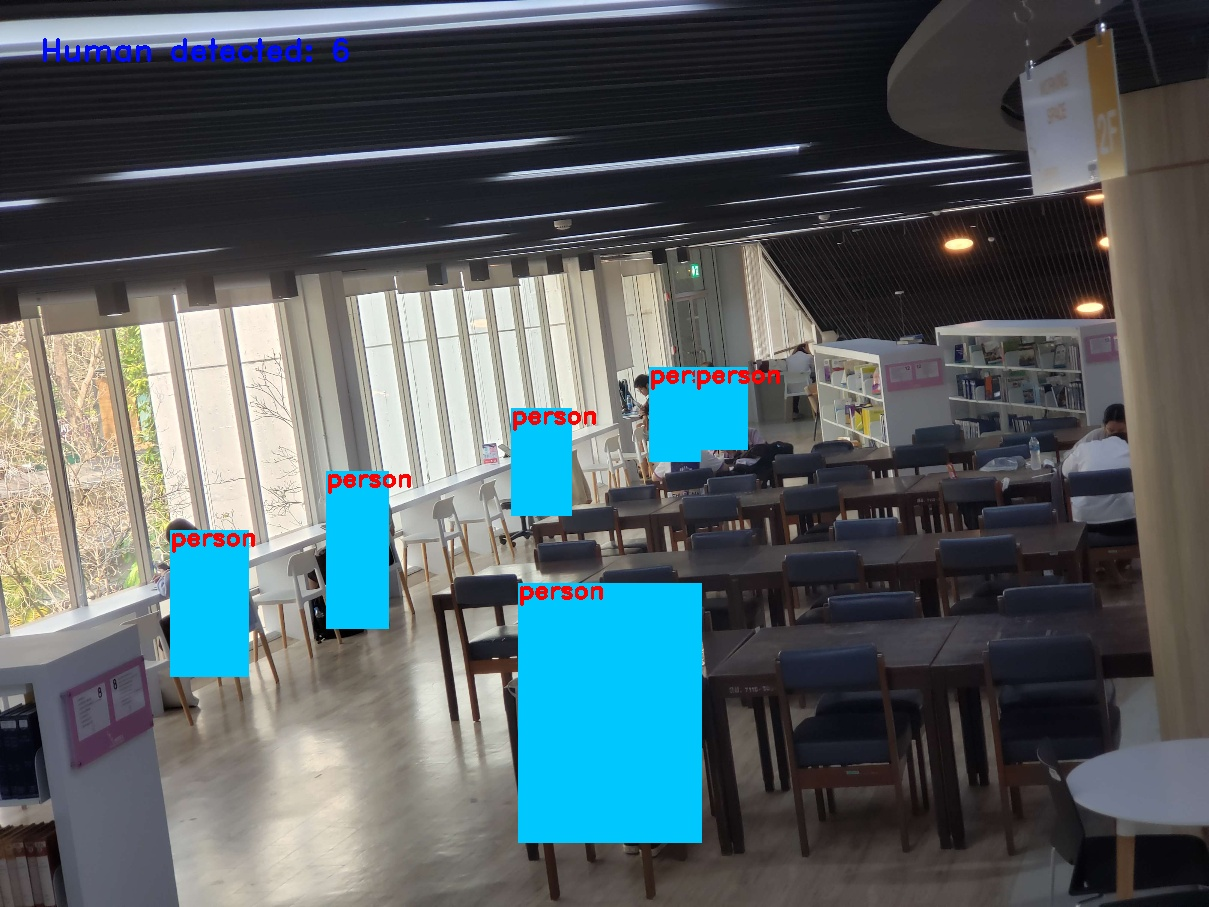
\includegraphics[scale=0.25]{images/dnn_output.jpg}
%     \caption[output 3]{output ของการทดลองครั้งที่ 3}
%     \label{fig:output3}
% \end{figure}
% ผลลัพธ์ที่ได้คือสามารถตรวจจับคนในภาพได้จำนวน 6 คน ซึ่งได้จำนวนน้อยกว่าความเป็นจริงเล็กน้อย มีความสามารถในการตรวจจับคนได้มากกว่าการทดลองครั้งที่ 2
% \section{สรุปผลการทดลอง}
% \hspace{10mm} จากผลการทดลองพบว่าการวิเคราะห์ผลของการทดลองครั้งที่ 3 โดยใช้ OpenCV DNN with TensorFlow ออกมาได้ค่อนข้างตรงที่สุด จึงคาดว่าจะใช้ model นี้ในการพัฒนาโครงงาน
% และในส่วนของการที่วิเคราะห์ผลออกมาผิดพลาดอาจเป็นเพราะมุมกล้อง ค่าสี ค่าความอิ่มตัวของสี หรือความสว่างของภาพที่อาจส่งผลต่อการวิเคราะห์ของ model จึงจะต้องมีการทดลองในส่วนนี้ต่อไป